%% aframe_gracedb_flow.tex  –  GraceDB submission data products and flow
%% Compile:  pdflatex aframe_gracedb_flow.tex && pdfcrop aframe_gracedb_flow.pdf
\documentclass{article}
\usepackage[margin=1cm, paperwidth=26cm, paperheight=24cm]{geometry}
\pagestyle{empty}
\usepackage{tikz}
\usetikzlibrary{positioning,arrows.meta,fit,backgrounds,calc}

\colorlet{mainfill}{blue!10}   \colorlet{mainbrd}{blue!55!black}
\colorlet{subfill} {orange!12} \colorlet{subbrd} {orange!65!black}
\colorlet{gdbfill} {purple!12} \colorlet{gdbbrd} {purple!55!black}
\colorlet{authfill}{gray!12}   \colorlet{authbrd}{gray!55}

\begin{document}
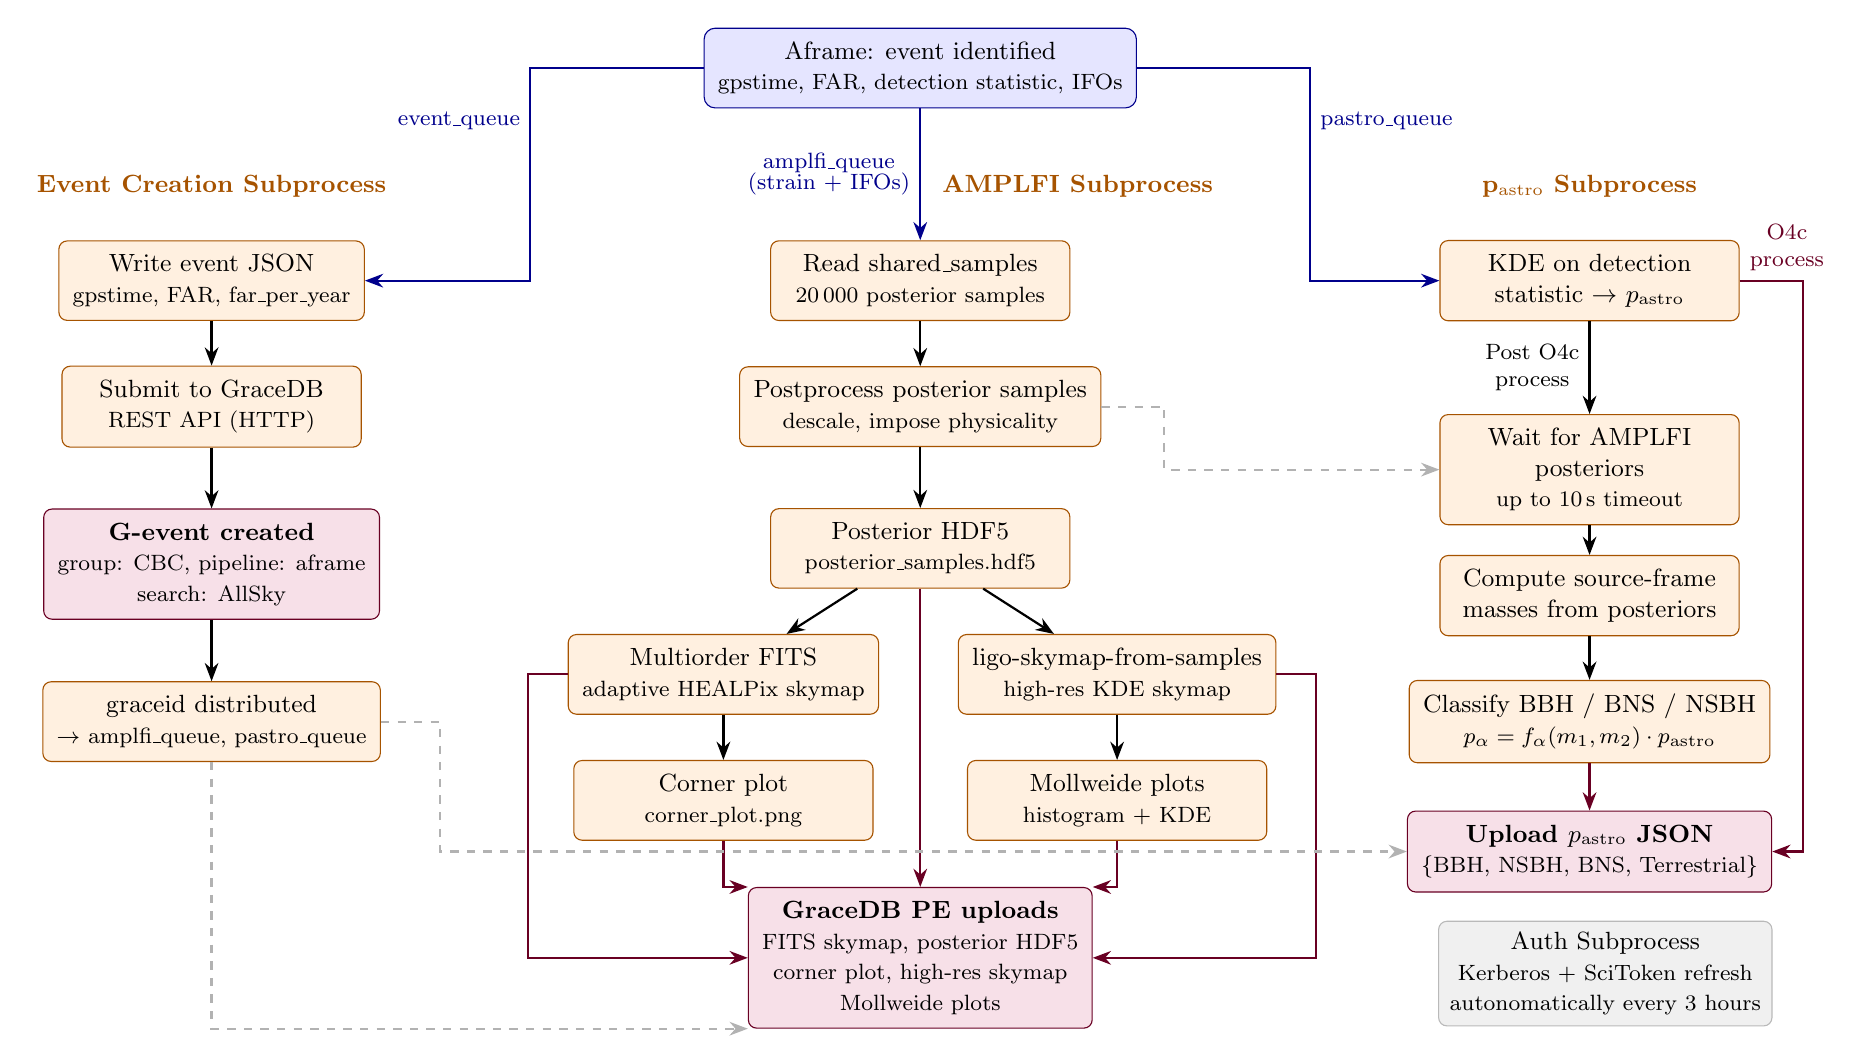
\begin{tikzpicture}[
  >=Stealth,
  every node/.style={font=\small, align=center},
  prod/.style  ={draw=subbrd, fill=subfill, rounded corners=3pt,
                 minimum width=3.8cm, minimum height=0.75cm, inner sep=5pt},
  gdb/.style   ={draw=gdbbrd, fill=gdbfill, rounded corners=3pt,
                 minimum width=3.8cm, minimum height=0.75cm, inner sep=5pt},
  trig/.style  ={draw=mainbrd, fill=mainfill, rounded corners=4pt,
                 minimum width=5.0cm, minimum height=0.9cm, inner sep=5pt},
  auth/.style  ={draw=authbrd, fill=authfill, rounded corners=3pt,
                 minimum width=3.6cm, minimum height=0.75cm, inner sep=4pt},
  sec/.style   ={font=\small\bfseries, subbrd},
  dep/.style   ={->, dashed, thick, gray!60},
  sub/.style   ={->, thick, gdbbrd},
  main/.style  ={->, thick, mainbrd},
]

%% ── Event trigger (top centre) ───────────────────────────────────────────
\node[trig] (trigger) at (11.5, 21.5)
  {Aframe: event identified\\{\footnotesize gpstime, FAR, detection statistic, IFOs}};

%% ════════════════════════════════════════════════════════════
%% LEFT COLUMN  –  Event Creation Subprocess   x ≈ 2.5
%% ════════════════════════════════════════════════════════════
\node[sec] at (2.5, 20.0) {Event Creation Subprocess};

\node[prod] (ev_json)  at (2.5, 18.8) {Write event JSON\\{\footnotesize gpstime, FAR, far\_per\_year}};
\node[prod] (ev_http)  at (2.5, 17.2) {Submit to GraceDB\\{\footnotesize REST API (HTTP)}};
\node[gdb]  (gdb_ev)   at (2.5, 15.2)
  {{\bfseries G-event created}\\{\footnotesize group: CBC, pipeline: aframe}\\{\footnotesize search: AllSky}};
\node[prod] (ev_gid)   at (2.5, 13.2)
  {graceid distributed\\{\footnotesize $\to$ amplfi\_queue, pastro\_queue}};

\draw[main] (trigger.west) -- ++(-2.2,0) |- node[very near start,left,font=\footnotesize]{event\_queue} (ev_json.east);
\draw[->, thick] (ev_json) -- (ev_http);
\draw[->, thick] (ev_http) -- (gdb_ev.north);
\draw[->, thick] (gdb_ev) -- (ev_gid);

%% ════════════════════════════════════════════════════════════
%% CENTRE COLUMN  –  AMPLFI Subprocess   x ≈ 11.5
%% ════════════════════════════════════════════════════════════
\node[sec] at (13.5, 20.0) {AMPLFI Subprocess};

\node[prod] (amp_samp)   at (11.5, 18.8)
  {Read shared\_samples\\{\footnotesize 20\,000 posterior samples}};
\node[prod] (amp_post)   at (11.5, 17.2)
  {Postprocess posterior samples\\{\footnotesize descale, impose physicality}};
\node[prod] (amp_hdf5)   at (11.5, 15.4)
  {Posterior HDF5\\{\footnotesize posterior\_samples.hdf5}};


\node[prod] (amp_fits)   at (9.0,  13.8)
  {Multiorder FITS\\{\footnotesize adaptive HEALPix skymap}};
\node[prod] (amp_corner) at (9, 12.2)
  {Corner plot\\{\footnotesize corner\_plot.png}};

\node[prod] (amp_lsky)   at (14.0,  13.8)
  {ligo-skymap-from-samples\\{\footnotesize high-res KDE skymap}};
\node[prod] (amp_mollw)  at (14.0, 12.2)
  {Mollweide plots\\{\footnotesize histogram + KDE}};

\draw[main] (trigger) -- node[left,font=\footnotesize]{amplfi\_queue\\[-2pt](strain + IFOs)} (amp_samp);
\draw[->, thick] (amp_samp) -- (amp_post);
\draw[->, thick] (amp_post) -- (amp_hdf5);
\draw[->, thick] (amp_hdf5) -- (amp_fits);
\draw[->, thick] (amp_fits) -- (amp_corner);
\draw[->, thick] (amp_hdf5) -- (amp_lsky);
\draw[->, thick] (amp_lsky) -- (amp_mollw);

% \draw[->, thick] (amp_fits.south) -- (amp_lsky.north);
% \draw[->, thick] (amp_hdf5.south) -- (amp_mollw.north);

%% AMPLFI uploads → GraceDB box
\node[gdb] (gdb_pe) at (11.5, 10.2)
  {{\bfseries GraceDB PE uploads}\\{\footnotesize FITS skymap, posterior HDF5}\\{\footnotesize corner plot, high-res skymap}\\{\footnotesize Mollweide plots}};

\draw[sub] (amp_hdf5)  -- (gdb_pe);
\draw[sub] (amp_fits.west)  -- ++(-0.5,0) |- (gdb_pe);
\draw[sub] (amp_lsky.east)  -- ++(0.5,0) |- (gdb_pe);
\draw[sub] (amp_corner.south) |- (gdb_pe.north west);
\draw[sub] (amp_mollw.south)  |- (gdb_pe.north east);

%% ════════════════════════════════════════════════════════════
%% RIGHT COLUMN  –  P_astro Subprocess   x ≈ 20.0
%% ════════════════════════════════════════════════════════════
\node[sec] at (20.0, 20.0) {p$_{\mathrm{astro}}$ Subprocess};

\node[prod] (pa_stat)  at (20.0, 18.8) {KDE on detection\\statistic $\to$ $p_{\mathrm{astro}}$};
\node[prod] (pa_post)  at (20.0, 16.4)
  {Wait for AMPLFI\\posteriors\\{\footnotesize up to 10\,s timeout}};
\node[prod] (pa_frac)  at (20.0, 14.8) {Compute source-frame\\masses from posteriors};
\node[prod] (pa_class) at (20.0, 13.2)
  {Classify BBH / BNS / NSBH\\{\footnotesize $p_{\alpha} = f_{\alpha}(m_1, m_2) \cdot p_{\mathrm{astro}}$}};
\node[gdb]  (gdb_pa)   at (20.0, 11.55)
  {{\bfseries Upload $p_{\mathrm{astro}}$ JSON}\\{\footnotesize \{BBH, NSBH, BNS, Terrestrial\}}};

\draw[main] (trigger.east) -- ++(2.2,0) |- node[very near start,right,font=\footnotesize]{pastro\_queue} (pa_stat.west);
\draw[->, thick] (pa_stat)  -- node[midway,left,font=\footnotesize]{Post O4c \\process} (pa_post);
\draw[->, thick] (pa_post)  -- (pa_frac);
\draw[->, thick] (pa_frac)  -- (pa_class);
\draw[sub]       (pa_class) -- (gdb_pa);

\draw[sub] (pa_stat.east) -- node[near end,above,font=\footnotesize]{O4c \\process} ++(0.8,0) |- (gdb_pa.east);

%% graceid → P_astro: route below ev_gid to avoid sharing AMPLFI dep segment
\draw[dep] (ev_gid.south) |- (gdb_pe.south west);
\draw[dep] (ev_gid.east) -- ++(0.75,0) |- (gdb_pa.west);

%% Posterior HDF5 from AMPLFI → P_astro wait
\draw[dep] (amp_post.east) -- ++(0.8,0) |- (pa_post.west);

%% ════════════════════════════════════════════════════════════
%% AUTH SUBPROCESS  –  below the main content, centred
%% ════════════════════════════════════════════════════════════
\node[auth] (authbox) at (20.2, 10.0)
  {Auth Subprocess\\{\footnotesize Kerberos + SciToken refresh}\\{\footnotesize autonomatically every 3 hours}};

\end{tikzpicture}
\end{document}
